\subsection{Memory Usage}
Apart from simulation execution time, memory usage during simulation is also of great importance.
While execution time only becomes a problem if it takes way too long, coming short only a bit of memory can make simulation unfeasible.
We therefore also investigate memory usage of different synchronization protocols, and again compare to adevs.

We do not tackle the problem of states that become too large for a single machine to hold.
This problem can be mitigated by distribution over multiple machines, which neither dxex or adevs support.

\subsubsection{Remarks}
Both dxex and adevs use \texttt{tcmalloc} as memory allocator, allowing for thread-local allocation.
Additionally, dxex uses memory pools to further reduce the frequency of expensive system calls (\textit{e.g.}, malloc and free).
\texttt{tcmalloc} only gradually releases memory back to the OS, whereas our pools will not do so at all.
Due to our motivation for memory usage analysis, we will only measure peak allocation in maximum resident set size as reported by the OS.

\subsubsection{Results}
Figure~\ref{fig:memory} shows the memory used by the different benchmarks.
Results are in megabytes, and show the total memory footprint of the running application (\textit{i.e.}, text, stack, and heap).

Unsurprisingly, optimistic synchronization results show very high memory usage due to the saved states.
Note the logarithmic scale that was used for this reason.
Optimistic synchronization results vary heavily depending on thread scheduling by the operating system, as this influences the drift between nodes.
Comparing similar approaches, we notice that dxex and adevs have very similar memory use.

Conservative simulation always uses more memory than sequential simulation, as is to be expected.
Additional memory is required for the multiple threads, but also to store all events that are processed simultaneously.

For the Phold benchmark, adevs using conservative synchronization took too long using our profiling tool, and was therefore aborted.
Therefore, no results are shown for adevs.

\begin{figure}
    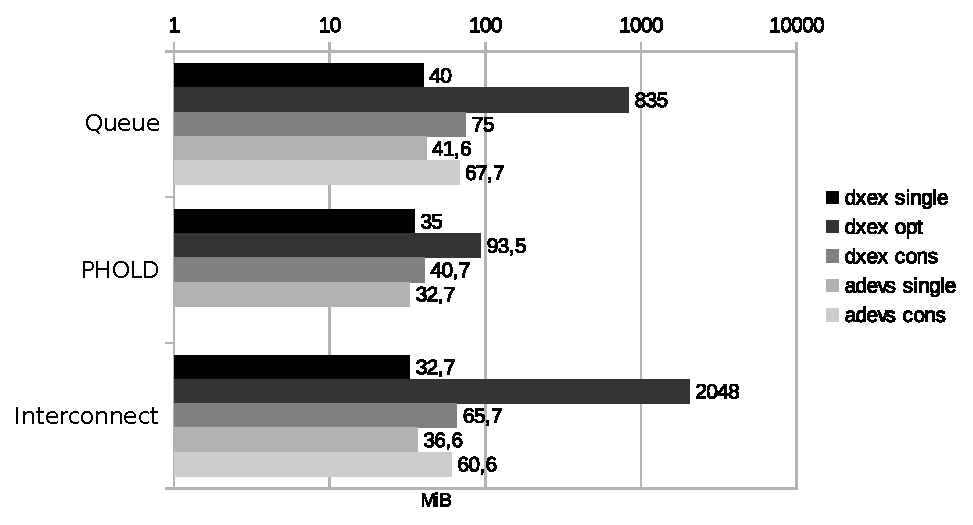
\includegraphics[width=\columnwidth]{fig/memory_voorlopig.eps}
    \caption{Memory usage results.}
    \label{fig:memory}
\end{figure}
